\documentclass{report}
\usepackage{listings}
\usepackage{graphicx}

\begin{document}
\title{Report 7 - Reduce}
\maketitle

\section{Grayscale}
\begin{lstlisting}[language=Python]
@c.jit
def grayscale(src, dst):
  tidx = c.threadIdx.x + c.blockIdx.x * c.blockDim.x
  tidy = c.threadIdx.y + c.blockIdx.y * c.blockDim.y

  if tidy < src.shape[0] and tidx < src.shape[1]:
    g = int((int(src[tidy, tidx, 0]) + int(src[tidy, tidx, 1]) + int(src[tidy, tidx, 2])) / 3)
    dst[tidy, tidx, 0] = dst[tidy, tidx, 1] = dst[tidy, tidx, 2] = g
\end{lstlisting}

\section{Reduce - compute min and max values}
\begin{lstlisting}[language=Python]
@c.jit
def reduce(dst, global_min, global_max):
  tidx = c.threadIdx.x + c.blockIdx.x * c.blockDim.x
  tidy = c.threadIdx.y + c.blockIdx.y * c.blockDim.y

  localtidx = c.threadIdx.x
  localtidy = c.threadIdx.y
\end{lstlisting}
I hardcoded the cuda shared array values as it was causing consistent GPU crashes in the past.
\begin{lstlisting}[language=Python]
  min_cache = c.shared.array((16, 16), numba.int32)
  max_cache = c.shared.array((16, 16), numba.int32)

  # copy local block from dst to cache (in shared memory)
  if tidy < dst.shape[0] and tidx < dst.shape[1]:
    min_cache[localtidy, localtidx] = dst[tidy, tidx, 0]
    max_cache[localtidy, localtidx] = dst[tidy, tidx, 0]
  else:
    min_cache[localtidy, localtidx] = 255
    max_cache[localtidy, localtidx] = 0
  
  c.syncthreads()
  # reduction in cache
  sy = int(c.blockDim.y / 2)
  sx = int(c.blockDim.x / 2)
\end{lstlisting}
The loop to move the min and max to index 0 of the cache
\begin{lstlisting}[language=Python]
  while sy > 0 and sx > 0:
    if (localtidy < sy) and (localtidx < sx):
      min_cache[localtidy, localtidx] = min(min_cache[localtidy, localtidx], min_cache[localtidy + sy, localtidx + sx])
      max_cache[localtidy, localtidx] = max(max_cache[localtidy, localtidx], max_cache[localtidy + sy, localtidx + sx])
    c.syncthreads()
    sx = sx // 2
    sy = sy // 2

\end{lstlisting}
These lines are to pass the values as global variables, i wasn't sure how to do it so I had to ask GenAI in english
\begin{lstlisting}[language=Python]
  c.atomic.min(global_min, 0, min_cache[0, 0])
  c.atomic.max(global_max, 0, max_cache[0, 0])
\end{lstlisting}

\section{Recalculating intensity}
\begin{lstlisting}[language=Python]
@c.jit
def recalculateIntensity(src, dst, g_min, g_max):
  tidx = c.threadIdx.x + c.blockIdx.x * c.blockDim.x
  tidy = c.threadIdx.y + c.blockIdx.y * c.blockDim.y
  local_min = g_min[0]
  local_max = g_max[0]
  if tidy < dst.shape[0] and tidx < dst.shape[1]:
    if local_max-local_min>0:
      g = int((src[tidy, tidx, 0]-local_min)*255/(local_max-local_min))
      dst[tidy, tidx, 0] = dst[tidy, tidx, 1] = dst[tidy, tidx, 2] = g
\end{lstlisting}

\section{Conclusion}
I had to manually lower the contrast of my image to see an actual change, so here are the 3 steps illustrated:
\begin{figure}[th]
    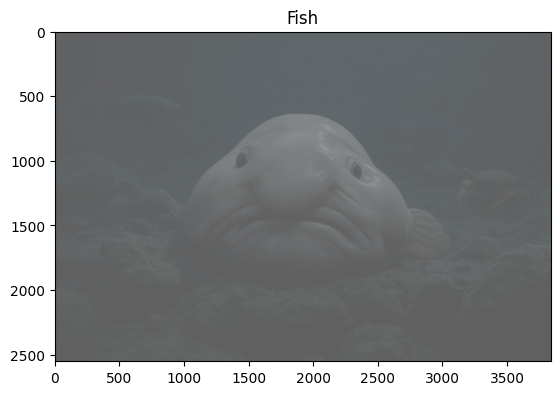
\includegraphics[width=0.5\linewidth]{first_fish.png}
    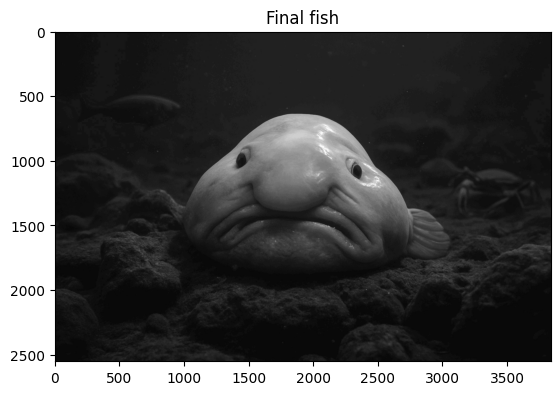
\includegraphics[width=0.5\linewidth]{New_fish.png}
\end{figure}
\end{document}
